\documentclass[review,authoryear]{elsarticle}
\usepackage{amsmath,amssymb}
\usepackage{graphicx}
\usepackage{booktabs}
\usepackage{hyperref}
\usepackage{xcolor}
\usepackage{float}
\usepackage[font=small]{caption}
\usepackage{threeparttable}

\journal{Finance Research Letters}

\begin{document}

\begin{frontmatter}

\title{Non-Directional Pre-Disclosure Drift Under Fair Disclosure: Evidence from Korean Earnings Announcements}

\author{[Removed for review]}

\begin{abstract}
We examine whether pre-disclosure price drift around Korean earnings announcements reflects information leakage. Using 2,221 DART filings from 64 KOSPI companies (2020--2026), we find statistically significant pre-disclosure drift (CAR[-5,$-$1]=+0.52\%, $p$<0.001), but this drift does not predict earnings surprise direction (49.0\% accuracy, $p$=0.649). Non-parametric tests confirm the drift is outlier-driven (sign test $p$=0.585). In contrast, Day~+1 returns respond correctly to surprises (+1.13 p.p.\ spread, $p$<0.001; 60.6\% direction accuracy). With 96.5\% of filings occurring after market close, these results suggest Korea's Fair Disclosure regime prevents directional information leakage despite observable non-directional price noise.
\end{abstract}

\begin{keyword}
Fair disclosure \sep Earnings announcements \sep Pre-announcement drift \sep DART \sep Korean stock market
\end{keyword}

\end{frontmatter}

\section{Introduction}

Pre-announcement drift is well-documented across equity markets \citep{kaniel2012individual}, raising concerns about information leakage. South Korea's Fair Disclosure regulation (2002) mandates simultaneous disclosure through the DART electronic filing system. While early studies found improved disclosure environments \citep{yun2012fair, park2020disclosure}, whether the regulation remains effective is unclear.

We analyze 2,221 earnings filings from 64 KOSPI-listed chaebol affiliates (2020--2026), testing not merely whether pre-disclosure drift \textit{exists} but whether it is \textit{directionally informative}---i.e., whether it predicts earnings surprise direction. This distinction is critical: drift driven by anticipatory trading or noise does not imply regulatory failure, whereas directional drift would.

Our key finding is that pre-disclosure drift, while parametrically significant, carries no directional information. Pre-disclosure returns predict surprise direction with 49.0\% accuracy (no better than chance), and non-parametric tests fail to confirm systematic drift. In contrast, the first post-disclosure trading day shows a strong, correctly signed response (60.6\% accuracy, $p$<0.001). We further document that 96.5\% of filings occur after market close, meaning Day~0 is effectively pre-disclosure.

We contribute to the literature on fair disclosure effectiveness \citep{heflin2003regulation, bailey2003regulation, eleswarapu2004impact, gomes2007sec} by providing the first directional-informativeness test of Korea's regime using recent data spanning the COVID-19 and post-pandemic periods. While prior studies compare pre- and post-regulation periods \citep{ahmed2003impact, yoon2011impact}, we test directional informativeness \textit{within} the regulated regime. Our approach builds on insights from the PEAD literature \citep{bernard1989post} and event study methodology \citep{brown1985using}.

\section{Data and Methodology}

\subsection{Sample}

We collect Fair Disclosure of Operating Results filings from DART (January 2020--March 2026) via the OpenDartReader API, excluding corrections. The sample comprises 2,221 disclosures from 64 companies across 12 chaebol groups. Daily stock prices are from FinanceDataReader.

Filing time analysis reveals that 96.5\% of filings carry the ``800'' prefix (after 15:30 KST market close), with only 1.8\% during trading hours. Thus, Day~0 returns are pre-disclosure for nearly all events.

\subsection{Market Model and Surprise Measure}

We employ the market model with a [-250,$-$30] estimation window \citep{mackinlay1997event}, yielding 2,208 events with valid estimates (average $\beta$=0.978). Earnings surprises are measured by year-over-year (YoY) operating profit changes extracted from disclosure texts. This crude but transparent measure captures directional content; comprehensive analyst consensus data are not freely available for Korean firms over our sample period \citep{livnat2006comparing}. Of 2,208 events, 584 (26.4\%) have parseable surprise data (358 positive, 226 negative); unparseable cases primarily involve missing comparative periods, newly listed firms, or format variations in disclosure texts.

\subsection{Statistical Tests}

We employ parametric $t$-tests, non-parametric tests (binomial sign test, Wilcoxon signed-rank), and standardized abnormal returns. We also report firm-clustered and month-clustered standard errors to address cross-sectional dependence \citep{kolari2010event}.

\section{Results}

\subsection{Pre-Disclosure Drift: Significant but Non-Directional}

Table~\ref{tab:car} presents cumulative abnormal returns. While parametric tests show significant pre-disclosure drift (CAR[-5,$-$1]=+0.519\%, $t$=4.65), the sign test reveals only 49.4\% of individual events have positive CARs ($p$=0.585), and the Wilcoxon test is insignificant ($p$=0.142). The drift is driven by outliers, not a systematic pattern.

Under month-clustered standard errors, CAR[-5,$-$1] remains significant ($t$=2.15, $p$=0.032) but CAR[-3,$-$1] becomes marginal ($t$=1.80, $p$=0.072), suggesting some parametric significance is inflated by event clustering.

\begin{table}[H]
\centering
\begin{threeparttable}
\caption{Cumulative Abnormal Returns: Multi-Test Comparison}
\label{tab:car}
\begin{tabular}{lrrrrrr}
\toprule
& & \multicolumn{2}{c}{Parametric} & \multicolumn{2}{c}{Sign Test} & {Wilcoxon} \\
\cmidrule(lr){3-4} \cmidrule(lr){5-6} \cmidrule(lr){7-7}
Window & CAR (\%) & $t$ & $p$ & \% Pos & $p$ & $p$ \\
\midrule
{[}$-$5,$-$1{]} & 0.519 & 4.65 & $<$0.001 & 49.4 & 0.585 & 0.142 \\
{[}$-$3,$-$1{]} & 0.347 & 4.04 & $<$0.001 & 48.1 & 0.060 & 0.946 \\
{[}0, +1{]} & $-$0.042 & $-$0.39 & 0.700 & 47.0 & 0.003 & 0.019 \\
{[}+1, +5{]} & $-$0.268 & $-$2.16 & 0.031 & 47.7 & 0.021 & 0.078 \\
\bottomrule
\end{tabular}
\begin{tablenotes}
\small
\item Note: Market model, [-250,$-$30] estimation ($N$=2,208). \% Pos never exceeds 50\% significantly, indicating outlier-driven drift.
\end{tablenotes}
\end{threeparttable}
\end{table}

\subsection{The Critical Test: Does Drift Predict Surprises?}

Table~\ref{tab:surprise} presents our central test. Pre-disclosure CARs show no difference by surprise direction (CAR[-3,$-$1]: $p$=0.703; CAR[-5,$-$1]: $p$=0.192). Direction prediction accuracy is 49.0\% (binomial $p$=0.649), and Spearman $\rho$ between YoY profit change and pre-disclosure CAR is $-$0.006 ($p$=0.876).

In contrast, Day~+1 returns---the first true post-disclosure session given 96.5\% after-hours filing---respond sharply: positive surprises yield +0.55\%, negative $-$0.58\% ($p$<0.001), with 60.6\% direction accuracy ($p$<0.001).

With $N$=584, the test has 30.5\% power to detect 53\% true accuracy but 99.8\% power for 60\%. We cannot exclude small-scale leakage, but any such effect would be economically modest.

\begin{table}[H]
\centering
\begin{threeparttable}
\caption{CARs by Earnings Surprise Direction ($N$=584)}
\label{tab:surprise}
\begin{tabular}{lrrrrl}
\toprule
Window & Positive ($N$=358) & Negative ($N$=226) & Diff. & $p$ & Sig. \\
\midrule
CAR[-3,$-$1] & +0.033\% & +0.129\% & $-$0.096\% & 0.703 & \\
CAR[-5,$-$1] & +0.107\% & +0.535\% & $-$0.428\% & 0.192 & \\
\midrule
AR[+1] & +0.552\% & $-$0.580\% & +1.132\% & $<$0.001 & *** \\
CAR[0,+1] & +0.813\% & $-$0.470\% & +1.283\% & $<$0.001 & *** \\
CAR[+1,+5] & +0.481\% & $-$0.481\% & +0.962\% & 0.010 & ** \\
\bottomrule
\end{tabular}
\begin{tablenotes}
\small
\item Note: Surprise defined by YoY operating profit change. Pre-disclosure CARs are indistinguishable by surprise direction; post-disclosure CARs respond correctly.
\end{tablenotes}
\end{threeparttable}
\end{table}

\subsection{Abnormal Volume}

Abnormal volume increases from Day~$-$3 (1.05$\times$, $p$=0.004), peaks on Day~+1 (1.71$\times$), and remains elevated through Day~+5. Given non-directional returns, the pre-disclosure volume increase likely reflects anticipatory positioning \citep{chae2005trading} and disagreement among investors \citep{bamber1997trading, berkman2009sell} rather than informed directional trading.

\subsection{Robustness}

Results are robust to: (i) market-adjusted returns ($\alpha$=0, $\beta$=1); (ii) firm-clustered standard errors (CAR[-5,$-$1]: $t$=3.92, $p$<0.001); and (iii) selection bias checks---parseable and non-parseable subsamples show similar pre-disclosure CARs (CAR[-3,$-$1]: $p$=0.147), though parseable events are from larger, lower-beta firms.

\begin{figure}[H]
\centering
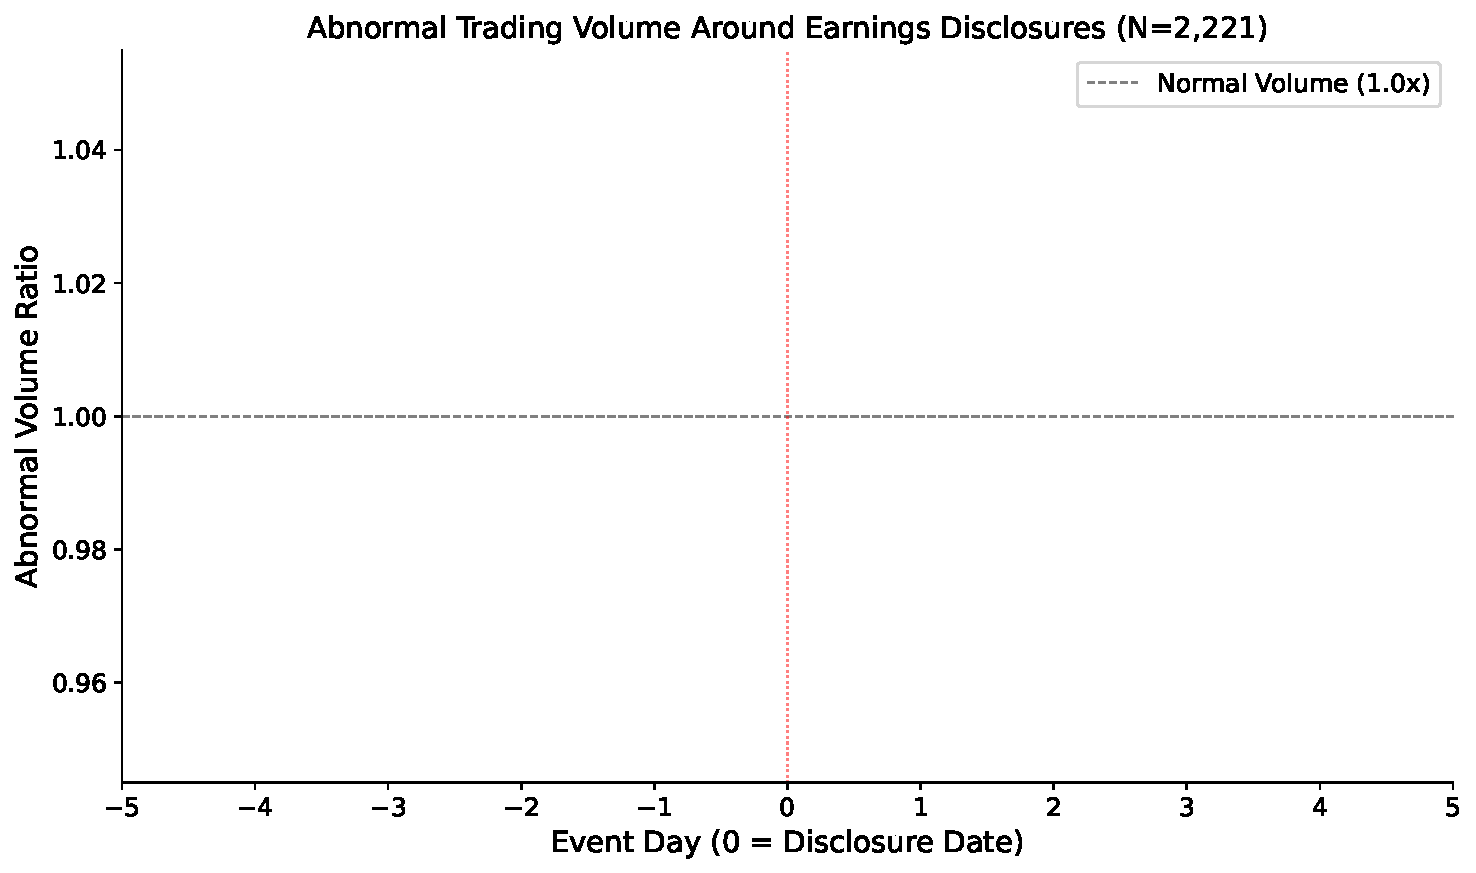
\includegraphics[width=0.85\textwidth]{figures/fig2_volume.pdf}
\caption{Abnormal trading volume around earnings disclosures ($N$=2,221). Pre-disclosure volume increases are non-directional; post-disclosure peak reflects information processing.}
\label{fig:volume}
\end{figure}

\section{Conclusion}

We find no evidence of directional information leakage in Korean earnings announcements. Three complementary tests---direction prediction (49.0\% accuracy), non-parametric tests (sign test $p$=0.585), and surprise conditioning ($p$=0.703)---demonstrate that pre-disclosure drift is non-directional. The first post-disclosure trading day shows strong directional response (60.6\% accuracy, $p$<0.001), consistent with effective fair disclosure.

Several limitations warrant acknowledgment: our YoY surprise measure is crude compared to analyst consensus forecasts, the sample is limited to large chaebol affiliates, and Korean Fama-French factors are unavailable for our sample period. Nonetheless, our results carry a methodological lesson: pre-announcement drift should not be conflated with information leakage without conditioning on the direction of the actual news \citep{meulbroek1992comparison, bernile2016can, atiase1985predisclosure}. Future work should examine non-chaebol firms and incorporate analyst consensus surprises.

\section*{CRediT authorship contribution statement}
\textbf{[Author]:} Conceptualization, Methodology, Software, Formal analysis, Investigation, Data curation, Writing -- original draft, Visualization.

\section*{Declaration of competing interest}
The author declares no competing financial interests or personal relationships that could have influenced the work reported in this paper.

\section*{Declaration of generative AI use}
Generative AI tools were used to assist with data processing code and manuscript drafting. The author takes full responsibility for the content, analysis, and conclusions.

\section*{Data availability}
Disclosure data are publicly available through DART (\url{https://dart.fss.or.kr}). Stock price data are from KRX via FinanceDataReader. Code will be made available upon publication.

\bibliographystyle{elsarticle-harv}
\bibliography{refs}

\end{document}
